\begin{tikzpicture}
\begin{scope}
\clip (0,.45) rectangle (8,7.8) ;
\node[anchor=south west,inner sep=0] at (0,0) {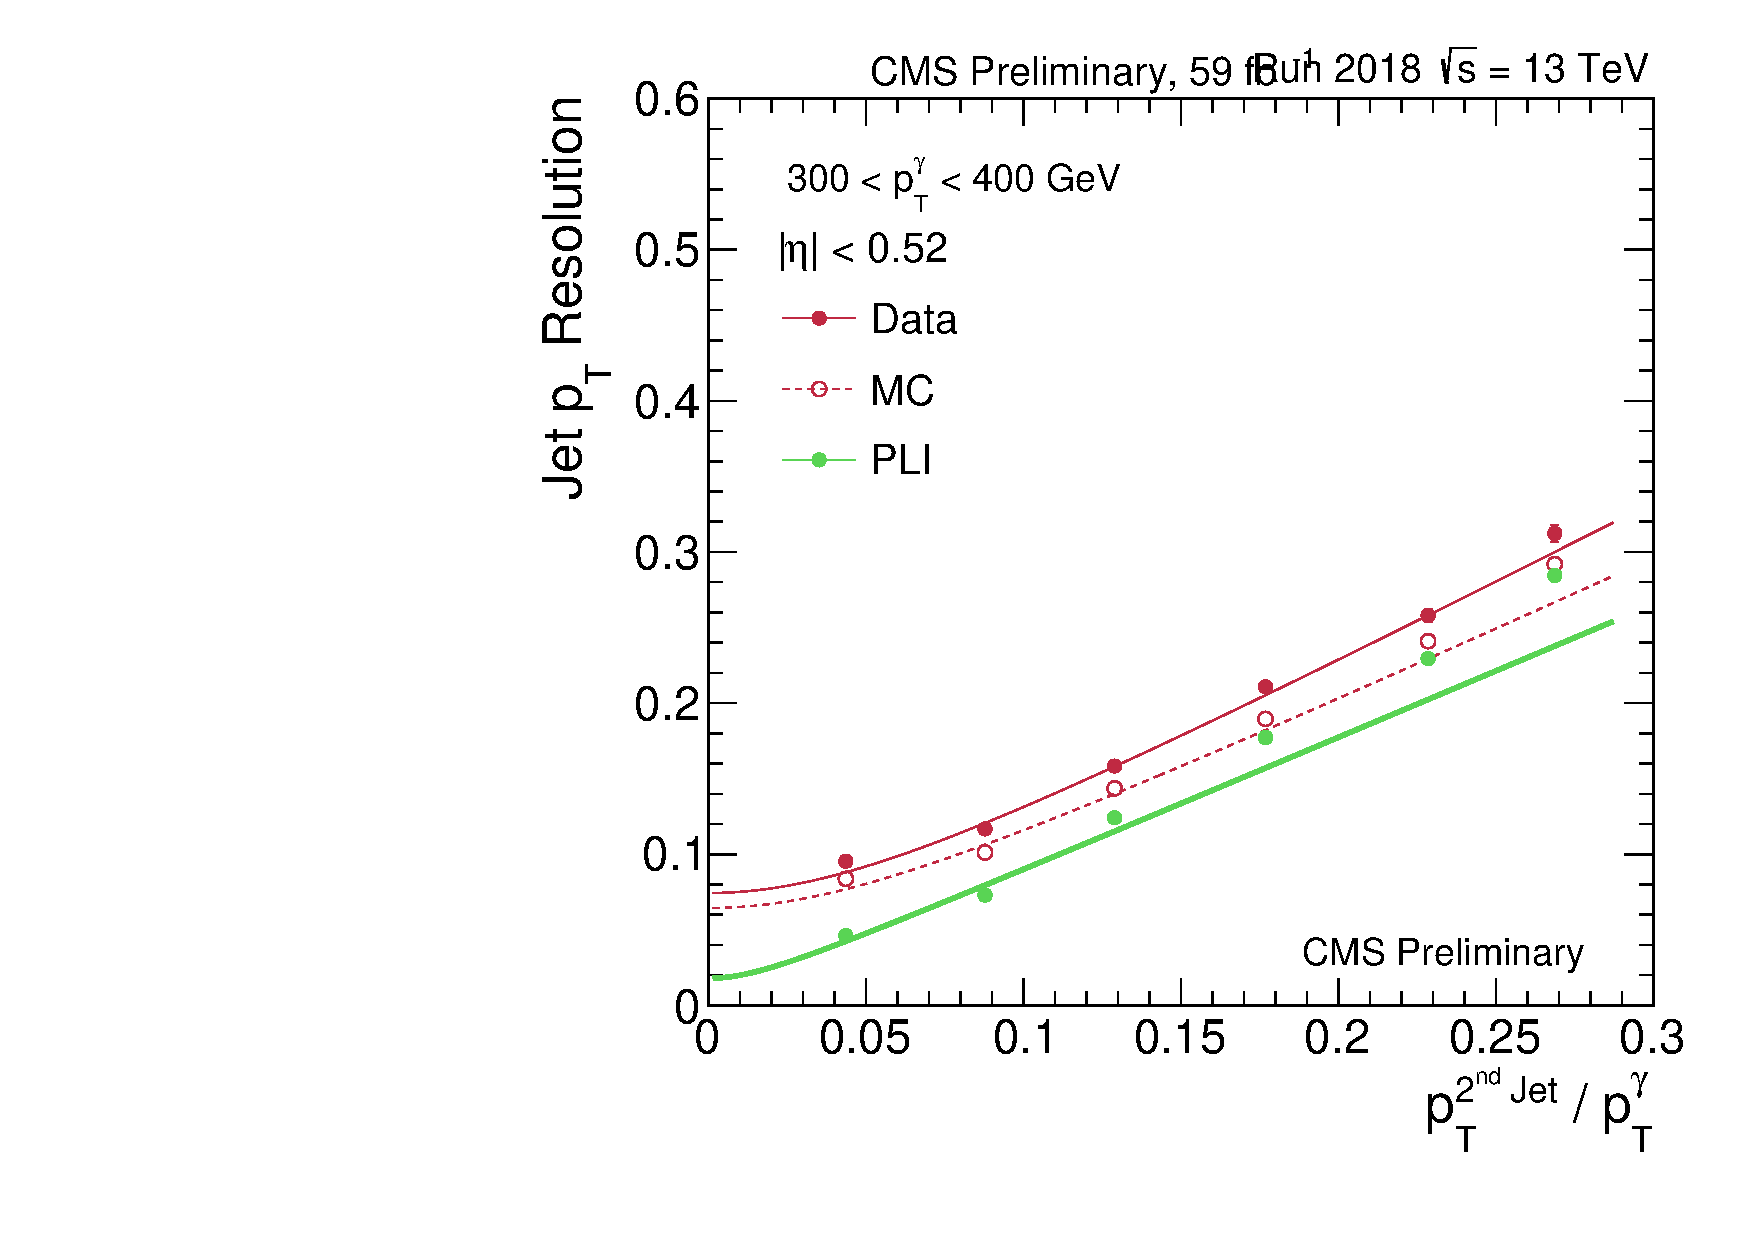
\includegraphics[width=8cm]{\PhDthesisdir/contents/chapter-JERC/plots/used/JER/Run2018ABCD/extrapolation/resolution_eta0005_ptPhot_300_400.pdf}};
\end{scope}

% masks
\fill [white] (1.2, 7.31) rectangle (7.6,7.7);
\fill [white] (1, 0.4) rectangle (7.85,1.1);
\fill [white] (0, 1) rectangle (1.15,7.5);
\clip (0,.4) rectangle (8,7.8) ;

% above txt
\draw (7.6, 7.5) node [left] {\footnotesize Run 2018 ABCD, \SI{59}{\femto\barn^{-1}} (\SI{13}{\TeV})};

% X axis
\foreach \val in {0, 0.05, 0.1, 0.15, 0.2, 0.25, 0.3}{
\draw ({1.2+(7.6-1.2)*\val/0.3}, .95) node {\small $\num{\val}$\vphantom{$\num{\val}\num{0.0}$}};
}
\draw (7, .5) node {$\alpha$};

% Y axis
\foreach \val in {0, 0.1, 0.2, 0.3, 0.4, 0.5, 0.6}{
\draw (1.25, {1.15+(7.25-1.15)*(\val)/(0.6)}) node [left] {\small $\num{\val}$};
}
\draw (.25, 7.25) node [left, rotate=90] {$\sigma$};
\end{tikzpicture}
